%*******************************************************%
%                                                        %
% William Cunningham                                    %
% wcunning@umich.edu                                    %
% EECS 470 -- Lab 1                                        %
%                                                        %
%*******************************************************%

%*******************************************************%
% Preamble                                                %
%*******************************************************%

\documentclass[table,dvipsnames,colorlinks=true]{beamer}
\usetheme{Lab}


\usepackage{
    siunitx,
    tikz,
    graphicx,
    amsmath,
    float,
    minted,
    hyperref,
    textcomp,
    circuitikz,
    xcolor,
    tikz-timing
}

\usepackage[T1]{fontenc}
%-----------------------%
% TikZ                    %
%-----------------------%
%--- CircuiTikZ Definitions ---%

%--- TikZ Definitions ---%
\usetikzlibrary{shapes,arrows,automata,shadows,circuits}
\pgfdeclarelayer{background}
\pgfdeclarelayer{foreground}
\pgfsetlayers{background,main,foreground}
% Block Diagram Styles
\tikzstyle{block} = [draw, fill=RoyalBlue!50, rounded corners, rectangle,
        minimum height=2cm, minimum width=2cm]
\tikzstyle{sum} = [draw, fill=blue!20, circle, node distance=2cm]
\tikzstyle{input} = [coordinate]
\tikzstyle{output} = [coordinate]
\tikzstyle{branch} = [coordinate]
\tikzstyle{pinstyle} = [pin edge={to-, thin, black}]
% Signal Flow Graph Styles
\tikzstyle{signal} = [draw, fill=blue!20, circle,
    minimum height=3em]

\definecolor{darkblue}{rgb}{0,0,0.8}

%*******************************************************%
% Document                                                %
%*******************************************************%

\title[Lab 1: Verilog]{EECS 470 Lab 1}
\subtitle{Verilog: Hardware Description Language}
\institute[University of Michigan]{Department of Electrical Engineering and 
            Computer Science \\
            College of Engineering \\
            University of Michigan}
%\author{William Cunningham \\ wcunning@umich.edu}
\date[January 21/22, 2021]{January 21/22, 2021}

\begin{document}
\frame{\titlepage}

\begin{frame}{Overview}
    \tableofcontents
\end{frame}

\section{EECS 470}
\begin{frame}{Help?}
    \begin{itemize}
        \item Contact Information
            \begin{itemize}
			 %   update with your info -- 
			    \item EECS 470 Staff Email - \href{mailto:@umich.edu}{eecs470w21staff@umich.edu } 
			    \item Emails sent to the above address will go to all instructors so we can respond to your questions faster.
				\item \href{https://piazza.com/umich/winter2021/eecs470}{\underline{EECS
                        470 Piazza}} (click for link)
                    \begin{itemize}
                        \item \href{https://piazza.com/class/kjoqguntyr139?cid=7}{\underline{Recordings}} can be found in a pinned Piazza Post.
                        \item Most of your project related questions should be
                            asked here so that other people can benefit from the
                            answer.
                        \item \textbf{Reminder:} Please do not post program code in public questions.
                    \end{itemize}
            \end{itemize}
        \item See up-to-date office hours on the
            %\href{put_calendar_here}{\underline{Google Calendar} (also linked on Canvas page)}
            \href{http://www.eecs.umich.edu/eecs/courses/eecs470}{\underline{course website}}.
        \end{itemize}
\end{frame}

\begin{frame}{Where? When?}
    \begin{itemize}        
    \item Due to the completely online nature
        \begin{itemize}
            \item Labs will be released shortly before the start of the first lab each week.
            \item A recording of the lab will be released at the end of each week.
            \item Please refer to the slides and recording for demonstrations and tips!
            \end{itemize}
    \item Lab attendance is optional but strongly recommended!
        \begin{itemize}
            \item Three Lab Sections
                \begin{itemize}
                    \item 011 -- Friday 10:30 am to 12:30 pm
                    \item 012 -- Thursday 6:00 pm to 8:00 pm
                    \item 013 -- Thursday 8:00 pm to 10:00 pm 
                \end{itemize}
            \item You can attend any of the lab sections. If the lab becomes very busy, please try to attend your own lab section hours (within reason). 
            \item Labs assignments must be checked off during a live meeting with an instructor. If you are unable to get checked off during lab, you can also get checked off during any office hours.
            \item Labs are due by the end of lab the week after they are assigned.
            \end{itemize}
    \end{itemize}
\end{frame}

\begin{frame}{What?}
    \begin{columns}
        \begin{column}[c]{0.8\textwidth}
            \begin{itemize}
                \item[Lab 1 --] Verilog: Hardware Description Language
                \item[Lab 2 --] The Build System
                \item[Lab 3 --] Writing Good Testbenches
                \item[Lab 4 --] Revision Control
                \item[Lab 5 --] Scripting
                \item[Lab 6 --] SystemVerilog
            \end{itemize}
        \end{column}
    \end{columns}
\end{frame}

\begin{frame}{Projects}
    \begin{columns}
        \begin{column}[c]{0.8\textwidth}
            \begin{block}{\hspace*{-32pt}Individual Verilog Projects}
            \begin{itemize}{\setlength\leftmargin{32pt}}
                    \item[Project 1 --] Priority Selectors (1\%)
                    \item[Project 2 --] Pipelined Multiplier, Integer Square Root (2\%)
                    \item[Project 3 --] Verisimple 5-stage Pipeline (5\%)
                \end{itemize}
            \end{block}
            \begin{block}{\hspace*{-32pt}Group Project}
                \begin{itemize}
                    \item[Project 4 --] Out-of-Order Processor (35\%)
                \end{itemize}
            \end{block}
        \end{column}
    \end{columns}
\end{frame}

\begin{frame}{Advice}
    \begin{itemize}
        \item These projects will take a non-trivial amount of time, especially
            if you're not a Verilog guru.
        \item You should start them early. Seriously\dots
        \item Especially Project 3!
    \end{itemize}
\end{frame}

\begin{frame}{Project 4}
    \begin{itemize}
        \item RISCV-V ISA
            \begin{itemize}
                \item An open source ISA that has commercial products
				\item Better software support, education friendly and has various extensions that include additinoal functionality
            \end{itemize}
        \item Groups of 4 to 5
            \begin{itemize}
                \item Start thinking about your groups now
                \item You'll be spending hundreds of hours together this
                    semester, so work with people with whom you get along.
            \end{itemize}
        \item Heavy Workload
            \begin{itemize}
                \item 100 hours/member, minimum
                \item 150 to 300 hours/member, more realistically
                \item This is a lower bound, not an upper bound\dots
            \end{itemize}
        \item Class is heavily loaded to the end of the term
    \end{itemize}
\end{frame}

\begin{frame}{Administrivia}
    \begin{itemize}
        \item Homework 1 is due Thursday, 4th$^{\text{th}}$ February, 2021 11:59 PM (turn in via Gradescope)
        \item Project 1 is due Friday, 29th$^{\text{th}}$ January, 2021 11:59 PM (turn in via submission script)
        \item  Lab 1 is due Friday, 29th$^{\text{th}}$ January, 2021 12:30 PM (live demo of your design to an instructor)
    \end{itemize}
\end{frame}

\section{Verilog}
\begin{frame}{Intro to Verilog}
    \begin{block}{What is Verilog?}
        \begin{itemize}
            \item Hardware Description Language - IEEE 1364-2005
                \begin{itemize}
                    \item Superseded by SystemVerilog - IEEE 1800-2009
                \end{itemize}
            \item Two Forms
                \begin{enumerate}
                    \item Behavioral
                    \item Structural 
                \end{enumerate}
            \item It can be built into hardware. If you can't think of at
                least one (inefficient) way to build it, it might not be
                good.
        \end{itemize}
    \end{block}
    \begin{block}{Why do I care?}
        \begin{itemize}
            \item We use Behavioral Verilog to do computer architecture here.
            \item Semiconductor Industry Standard (VHDL is also common, more so in Europe)
        \end{itemize}
    \end{block}
\end{frame}

\begin{frame}{The Difference Between Behavioral and Structural Verilog}
    \begin{columns}
        \begin{column}[T]{0.45\textwidth}
            \begin{block}{Behavioral Verilog}
                \begin{itemize}
                    \item Describes function of design 
                    \item Abstractions
                        \begin{itemize}
                            \item Arithmetic operations (\texttt{+,-,*,/})
                            \item Logical operations
                                (\texttt{\&,|,\^{},\char`\~})
                        \end{itemize}
                \end{itemize}
            \end{block}
        \end{column}
        \begin{column}[T]{0.45\textwidth}
            \begin{block}{Structural Verilog}
                \begin{itemize}
                    \item Describes construction of design
                    \item No abstraction
                    \item Uses modules, corresponding to physical devices, for everything 
                \end{itemize}
            \end{block}
        \end{column}
    \end{columns}
    \begin{block}{}
        \center{Suppose we want to build an adder?}
    \end{block}
\end{frame}

\begin{frame}{Structural Verilog by Example}
    \begin{figure}[h]
        \begin{circuitikz}[scale=1]
            \draw (1,3.5) node[xor port] (xor1) {};
            \draw (4,3) node[xor port] (xor2) {};
            \draw (4,1.5) node[and port] (and1) {};
            \draw (4,0) node[and port] (and2) {};
            \draw (6,0.75) node[or port] (or1) {};

            \draw (xor1.in 1)+(-1,0) node[anchor=east] {\texttt{a}$\circ$};
            \draw (xor1.in 1) -- +(-1.15,0);
            \draw (xor1.in 2)+(-1,0) node[anchor=east] {\texttt{b}$\circ$};
            \draw (xor1.in 2) -- +(-1.15,0);
            \draw (and1.out) -| node[anchor=south,pos=0.1] {\texttt{w\_1}} (or1.in 1);
            \draw (and2.out) -| node[anchor=south,pos=0.1] {\texttt{w\_2}} (or1.in 2);
            \draw (xor2.in 1) -- node[pos=0.5,anchor=south] {\texttt{w\_0}} +(-1,0) -- (xor1.out);
            \draw (xor2.in 2)+(-4,0) node[anchor=east] {\texttt{cin}$\circ$};
            \draw (xor2.in 2) -- +(-4.15,0);
            \draw (xor2.in 1)+(-0.5,0) node[circ] {} |- (and1.in 1);
            \draw (xor2.in 2)+(-1,0) node[circ] {} |- (and1.in 2);
            \draw (xor1.in 1)+(-0.25,0) node[circ] {} |- (and2.in 1);
            \draw (xor1.in 2)+(-0.75,0) node[circ] {} |- (and2.in 2);

            \draw (xor2.out) -- +(2.25,0);
            \draw (xor2.out)+(2.1,0)node[anchor=west] {$\circ$\texttt{s}}; 
            \draw (or1.out) -- +(0.25,0);
            \draw (or1.out)+(0.1,0)node[anchor=west] {$\circ$\texttt{cout}}; 

            \draw (xor1)+(-0.25,0) node[anchor=east] {\texttt{u0}};
            \draw (xor2)+(-0.25,0) node[anchor=east] {\texttt{u1}};
            \draw (and1)+(-0.25,0) node[anchor=east] {\texttt{u2}};
            \draw (and2)+(-0.25,0) node[anchor=east] {\texttt{u3}};
            \draw (or1)+(-0.25,0) node[anchor=east] {\texttt{u4}};
        \end{circuitikz}
        \caption{1-bit Full Adder}
    \end{figure}
\end{frame}

\begin{frame}[fragile]{Structural Verilog by Example}
    \begin{minted}[frame=lines,fontsize=\footnotesize]{verilog}
        module one_bit_adder(
            input wire a,b,cin,
            output wire sum,cout);
            wire w_0,w_1,w_2;
            xor u0(w_0,a,b);
            xor u1(sum,w_0,cin);
            and u2(w_1,w_0,cin);
            and u3(w_2,a,b);
            or u4(cout,w_1,w_2);
        endmodule
    \end{minted}
\end{frame}

\begin{frame}[fragile]{Behavioral Verilog by Example}
    \begin{minted}[frame=lines,fontsize=\footnotesize]{verilog}
        module one_bit_adder(
            input wire a,b,cin,
            output wire sum,cout);
            assign sum = a ^ b ^ cin;
            assign cout = ((a ^ b) & cin) | a & b;
        endmodule
    \end{minted}
\end{frame}

\begin{frame}[fragile]{Behavioral Verilog by Example}
    \begin{minted}[frame=lines,fontsize=\footnotesize]{verilog}
        module one_bit_adder(
            input logic a,b,cin,
            output logic sum,cout);
            
            always_comb
            begin
                sum = a ^ b ^ cin;
                cout = 1'b0;
                if ((a ^ b) & cin) | (a & b))
                    cout = 1'b1;
            end
        endmodule
    \end{minted}
\end{frame}

\begin{frame}{Verilog Semantics}
    \begin{block}{Lexical}
        \begin{itemize}
            \item Everything is case sensitive.
            \item Type instances must start with \texttt{A-Z,a-z,\_}. They may
                contain \texttt{A-Z,a-z,0-9,\_,\$}. 
            \item Comments begin with \texttt{//} or are enclosed with
                \texttt{/*} and \texttt{*/}.
        \end{itemize}
    \end{block}
\end{frame}

\begin{frame}[fragile]{Data Types}
    \begin{columns}
        \begin{column}[T]{0.85\textwidth}
            \begin{block}{Synthesizable Data Types}
                \begin{itemize}
                    \item[\texttt{wires}] Also called nets
                        \begin{minted}[frame=lines,fontsize=\footnotesize]{verilog}
                wire a_wire;
                wire [3:0] another_4bit_wire;
                        \end{minted}
                        \begin{itemize}
                            \item Cannot hold state
                        \end{itemize}
                    \item[\texttt{logic}] Replaced \texttt{reg} in SystemVerilog
                        \begin{minted}[frame=lines,fontsize=\footnotesize]{verilog}
                logic [7:0] an_8bit_register;    
                reg a_register;
                        \end{minted}
                        \begin{itemize}
                            \item Holds state, might turn into flip-flops
                            \item Less confusing than using \texttt{reg} with
                                combinational logic (coming up\dots)
                        \end{itemize}
                \end{itemize}
            \end{block}
        \end{column}
    \end{columns}
\end{frame}

\begin{frame}{Data Types}
    \begin{columns}
        \begin{column}[T]{0.85\textwidth}
            \begin{block}{Unsynthesizable Data Types}
                \begin{itemize}
                    \item[\texttt{integer}] Signed 32-bit variable
                    \item[\texttt{time}] Unsigned 64-bit variable
                    \item[\texttt{real}] Double-precision floating point variable
                \end{itemize}
            \end{block}
        \end{column}
    \end{columns}
\end{frame}

\begin{frame}{Types of Values}
    \begin{block}{Four State Logic}
        \begin{itemize}
            \item[\texttt{0}] False, low
            \item[\texttt{1}] True, high
            \item[\texttt{Z}] High-impedance, unconnected net
            \item[\texttt{X}] Unknown, invalid, don't care
        \end{itemize}
    \end{block}
\end{frame}

\begin{frame}[fragile]{Values}
    \begin{block}{Literals/Constants}
        \begin{itemize}
            \item Written in the format \texttt{<bitwidth>'<base><constant>}
            \item Options for \texttt{<base>} are\dots
                \begin{itemize}
                    \item[\texttt{b}] Binary
                    \item[\texttt{o}] Octal
                    \item[\texttt{d}] Decimal
                    \item[\texttt{h}] Hexadecimal
                \end{itemize}
                \begin{minted}[frame=lines,fontsize=\footnotesize]{verilog}
                    assign an_8bit_register = 8'b10101111;
                    assign a_32bit_wire = 32'hABCD_EF01;
                    assign a_4bit_logic = 4'hE;
                \end{minted}
        \end{itemize}
    \end{block}
\end{frame}

\begin{frame}{Verilog Operators}
    \footnotesize
    \begin{columns}
        \hspace*{-36pt}
        \begin{column}[T]{0.55\textwidth}
            \vspace*{-18pt}
            \begin{table}[h]
                \begin{tabular}{rl}
                     \rowcolor{RoyalBlue!50}
                    \multicolumn{2}{c}{Arithmetic} \\  
                    \rowcolor{RoyalBlue!20}
                    \texttt{*} & Multiplication \\ 
                    \rowcolor{RoyalBlue!20}
                    \texttt{/} & Division \\
                    \rowcolor{RoyalBlue!20}
                    \texttt{+} & Addition \\
                    \rowcolor{RoyalBlue!20}
                    \texttt{-} & Subtraction \\
                    \rowcolor{RoyalBlue!20}
                    \texttt{\%} & Modulus \\
                    \rowcolor{RoyalBlue!20}
                    \texttt{**} & Exponentiation \\
                     \rowcolor{RoyalBlue!50}
                    \multicolumn{2}{c}{Bitwise} \\ 
                    \rowcolor{RoyalBlue!20}
                    \texttt{\char`\~} & Complement \\
                    \rowcolor{RoyalBlue!20}
                    \texttt{\&} & And \\
                    \rowcolor{RoyalBlue!20}
                    \texttt{|} & Or \\
                    \rowcolor{RoyalBlue!20}
                    \texttt{\char`\~|} & Nor \\
                    \rowcolor{RoyalBlue!20}
                    \texttt{\^{}} & Xor \\
                    \rowcolor{RoyalBlue!20}
                    \texttt{\char`\~\^{}} & Xnor \\
                     \rowcolor{RoyalBlue!50}
                    \multicolumn{2}{c}{Logical} \\  
                    \rowcolor{RoyalBlue!20}
                    \texttt{!} & Complement \\
                    \rowcolor{RoyalBlue!20}
                    \texttt{\&\&} & And \\
                    \rowcolor{RoyalBlue!20}
                    \texttt{||} & Or \\
                \end{tabular}
            \end{table}
        \end{column}
        \hspace*{-84pt}
        \begin{column}[T]{0.55\textwidth}
            \vspace*{-18pt}  
            \begin{table}[h]
                \begin{tabular}{rl}
                     \rowcolor{RoyalBlue!50}
                    \multicolumn{2}{c}{Shift} \\  
                    \rowcolor{RoyalBlue!20}
                    \texttt{\textgreater{\textgreater}} & Logical right shift \\
                    \rowcolor{RoyalBlue!20}
                    \texttt{\textless{\textless}} & Logical left shift \\
                    \rowcolor{RoyalBlue!20}
                    \texttt{\textgreater{\textgreater}\textgreater} & Arithmetic right shift \\
                    \rowcolor{RoyalBlue!20}
                    \texttt{\textless{\textless}\textless} & Arithmetic left shift \\
                     \rowcolor{RoyalBlue!50}
                    \multicolumn{2}{c}{Relational} \\  
                    \rowcolor{RoyalBlue!20}
                    \texttt{>} & Greater than \\
                    \rowcolor{RoyalBlue!20}
                    \texttt{>=} & Greater than or equal to \\
                    \rowcolor{RoyalBlue!20}
                    \texttt{<} & Less than \\
                    \rowcolor{RoyalBlue!20}
                    \texttt{<=} & Less than or equal to \\
                    \rowcolor{RoyalBlue!20}
                    \texttt{!=} & Inequality \\
                    \rowcolor{RoyalBlue!20}
                    \texttt{!==} & 4-state inequality \\
                    \rowcolor{RoyalBlue!20}
                    \texttt{==} & Equality \\
                    \rowcolor{RoyalBlue!20}
                    \texttt{===} & 4-state equality \\
                     \rowcolor{RoyalBlue!50}
                    \multicolumn{2}{c}{Special} \\  
                    \rowcolor{RoyalBlue!20}
                    \texttt{\{,\}} & Concatenation \\
                    \rowcolor{RoyalBlue!20}
                    \texttt{\{n\{m\}\}} & Replication \\
                    \rowcolor{RoyalBlue!20}
                    \texttt{?:} & Ternary \\
                \end{tabular}
            \end{table}
        \end{column}
    \end{columns}
\end{frame}

\begin{frame}[fragile]{Setting Values}
    \begin{block}{\texttt{assign} Statements}
        \begin{itemize}
            \item One line descriptions of combinational logic
            \item Left hand side must be a wire (SystemVerilog allows assign statements on logic type)
            \item Right hand side can be any one line verilog expression
            \item Including (possibly nested) ternary (\texttt{?:})
        \end{itemize}
    \end{block}
    \begin{block}{Example}
        \begin{minted}[frame=lines,fontsize=\footnotesize]{verilog}
            module one_bit_adder(
                input wire a,b,cin,
                output wire sum,cout);
                assign sum = a ^ b ^ cin;
                assign cout = ((a ^ b) & cin) | a & b;
            endmodule
        \end{minted}
    \end{block}
\end{frame}

\begin{frame}{Setting Values}
    \begin{block}{\texttt{always} Blocks}
        \begin{itemize}
            \item Contents of \texttt{always} blocks are executed whenever
                anything in the sensitivity list happens
            \item Two main types in this class\dots
                \begin{itemize}
                    \item \texttt{always\_comb}
                        \begin{itemize}
                            \item implied sensitivity lists of every signal 
                                inside the block
                            \item Used for combinational logic. Replaced 
                                \texttt{always @*}
                        \end{itemize}
                    \item \texttt{always\_ff @(posedge clk)} 
                        \begin{itemize}
                            \item sensitivity list containing only the positive 
                                transition of the \texttt{clk} signal
                            \item Used for sequential logic
                        \end{itemize}
                \end{itemize}
            \item All left hand side signals need to be \texttt{logic} type.
        \end{itemize}
    \end{block}
\end{frame}

\begin{frame}[fragile]{Always Block Examples}
    \begin{block}{Combinational Block}
        \begin{minted}[frame=lines,fontsize=\footnotesize]{verilog}
            always_comb
            begin
                x = a + b;
                y = x + 8'h5;
            end
        \end{minted}
    \end{block}
    \begin{block}{Sequential Block}
        \begin{minted}[frame=lines,fontsize=\footnotesize]{verilog}
            always_ff @(posedge clk)
            begin
                x <= #1 next_x;
                y <= #1 next_y;
            end
        \end{minted}
    \end{block}
\end{frame}

\begin{frame}{Blocking vs. Nonblocking Assignments}
    \begin{columns}
        \begin{column}[T]{0.45\textwidth}
            \begin{block}{Blocking Assignment}
                \begin{itemize}
                    \item Combinational Blocks
                    \item Each assignment is processed in order, earlier
                        assignments block later ones
                    \item Uses the \texttt{=} operator
                \end{itemize}
            \end{block}
        \end{column}
        \begin{column}[T]{0.05\textwidth}
            \vspace*{0.25\textheight}
            \Large{vs.}
            \normalsize
        \end{column}
        \begin{column}[T]{0.45\textwidth}
            \begin{block}{Nonblocking Assignment}
                \begin{itemize}
                    \item Sequential Blocks
                    \item All assignments occur ``simultaneously,'' delays are
                        necessary for accurate simulation
                    \item Uses the \texttt{<=} operator
                \end{itemize}
            \end{block}
        \end{column}
    \end{columns}
\end{frame}

\begin{frame}[fragile]{Blocking vs. Nonblocking Assignment by Example}
    \begin{block}{Blocking Example}
        \vspace*{-12pt}
        \begin{minted}[frame=lines,fontsize=\footnotesize]{verilog}
            always_comb
            begin
                x = new_val1;
                y = new_val2;
                sum = x + y;
            end
        \end{minted}
    \end{block}
    \vspace*{-18pt}
    \begin{columns}
        \begin{column}[T]{0.45\textwidth}
            \begin{itemize}
                \item Behave exactly as expected
                \item Standard combinational logic
            \end{itemize}
        \end{column}
        \begin{column}[T]{0.45\textwidth}
            \vspace*{-6pt}
            \begin{figure}[h]
                \begin{tikztimingtable}
                    \texttt{new\_val1} & LHLHLHLHLH \\ 
                    \texttt{x} & LHLHLHLHLH \\
                    \texttt{new\_val2} & LLHHLLHHLL \\
                    \texttt{y} & LLHHLLHHLL \\
                    \texttt{sum} & LHHLLHHLLH\\
                    \extracode
                        \begin{pgfonlayer}{background}
                            \vertlines[blue!50]{1,2,...,10}
                        \end{pgfonlayer}
                \end{tikztimingtable}
                \caption{Timing diagram for the above example.}
            \end{figure}
        \end{column}
    \end{columns}
\end{frame}

\begin{frame}[fragile]{Blocking vs. Nonblocking Assignment by Example}
    \begin{block}{Nonblocking Example}
        \vspace*{-12pt}
        \begin{minted}[frame=lines,fontsize=\footnotesize]{verilog}
            always_ff @(posedge clock)
            begin
                x <= #1 new_val1;
                y <= #1 new_val2;
                sum <= #1 x + y;
            end
        \end{minted}
    \end{block}
    \vspace*{-18pt}
    \begin{columns}
        \begin{column}[T]{0.4\textwidth}
            \begin{itemize}
                \item What changes between these two examples?
                \item Nonblocking means that \texttt{sum} lags a cycle behind
                    the other two signals
            \end{itemize}
        \end{column}
        \begin{column}[T]{0.65\textwidth}
            \vspace*{-6pt}
            \begin{figure}[h]
                \begin{tikztimingtable}
                    \texttt{clock} & 16{C} \\
                    \texttt{new\_val1} & LLHHLLHHLLHHLLHH \\ 
                    \texttt{x} & XLLHHLLHHLLHHLLH \\
                    \texttt{new\_val2} & LLLLHHHHLLLLHHHH \\
                    \texttt{y} & XLLLLHHHHLLLLHHH \\
                    \texttt{sum} & XXLLLHHHHLLLLHHH \\
                    \extracode
                        \begin{pgfonlayer}{background}
                            \vertlines[blue!50]{1,2,...,16}
                        \end{pgfonlayer}
                \end{tikztimingtable}
                \caption{Timing diagram for the above example.}
            \end{figure}
        \end{column}
    \end{columns}
\end{frame}

\begin{frame}[fragile]{Blocking vs. Nonblocking Assignment by Example}
    \begin{block}{Bad Example}
        \vspace*{-12pt}
        \begin{minted}[frame=lines,fontsize=\footnotesize]{verilog}
            always_ff @(posedge clock)
            begin
                x <= #1 y;
                z = x;
            end
        \end{minted}
    \end{block}
    \vspace*{-18pt}
    \begin{columns}
        \begin{column}[T]{0.45\textwidth}
            \begin{itemize}
                \item \texttt{z} is updated after \texttt{x}
                \item \texttt{z} updates on \texttt{negedge clock}
            \end{itemize}
        \end{column}
        \begin{column}[T]{0.45\textwidth}
            \vspace*{-6pt}
            \begin{figure}[h]
                \begin{tikztimingtable}
                    \texttt{clock} & 10{C} \\
                    \texttt{reset} & HHHLLLLLLL \\
                    \texttt{x} & XXLLLLHHLL \\
                    \texttt{y} & LLLHHLLLLL \\
                    \texttt{z} & XXXXLLLLHH \\
                    \extracode
                        \begin{pgfonlayer}{background}
                            \vertlines[blue!50]{1,2,...,10}
                        \end{pgfonlayer}
                \end{tikztimingtable}
                \caption{Timing diagram for the above example.}
            \end{figure}
        \end{column}
    \end{columns}
\end{frame}

\begin{frame}{Synthesis Tips}
    \begin{block}{Latches}
        \begin{itemize}
            \item What is a latch?
                \begin{itemize}
                    \item Memory device without a clock
                \end{itemize}
            \item Generated by a synthesis tool when a net needs to hold
                state without being clocked (combinational logic)
            \item Generally bad, unless designed in intentionally
            \item Unnecessary in this class
        \end{itemize}
    \end{block}
\end{frame}

\begin{frame}[fragile]{Synthesis Tips}
    \begin{block}{Latches}
        \begin{itemize}
            \item Always assign every variable on every path
            \item This code generates a latch
            \item Why does this happen?
        \end{itemize}
        \begin{minted}[frame=lines,fontsize=\footnotesize]{verilog}
            always_comb
            begin
                if (cond)
                    next_x = y;
            end
        \end{minted}
    \end{block}
\end{frame}

\begin{frame}[fragile]{Synthesis Tips}
    \begin{block}{Possible Solutions to Latches}
        \vspace*{-12pt}
        \begin{minted}[frame=lines,fontsize=\footnotesize]{verilog}
            always_comb
            begin
                next_x = x;
                if (cond)
                    next_x = y;
            end
        \end{minted}
        \begin{minted}[frame=lines,fontsize=\footnotesize]{verilog}
            always_comb
            begin
                if (cond)
                    next_x = y;
                else
                    next_x = x;
            end
        \end{minted}
    \end{block}
\end{frame}

\begin{frame}[fragile]{Modules}
    \begin{block}{Intro to Modules}
        \begin{itemize}
            \item Basic organizational unit in Verilog
            \item Can be reused
        \end{itemize}
    \end{block}
    \begin{block}{Module Example}
        \begin{minted}[frame=lines,fontsize=\footnotesize]{verilog}
            module my_simple_mux(
                input wire select_in, a_in, b_in; //inputs listed
                output wire muxed_out); //outputs listed
                assign muxed_out = select_in ? b_in : a_in;
            endmodule
        \end{minted}
    \end{block}
\end{frame}

\begin{frame}{Modules}
    \begin{block}{Writing Modules}
        \begin{itemize}
            \item Inputs and outputs must be listed, including size and type \\
                format: \texttt{<dir> <type> <[WIDTH-1:0]> <name>;} \\
                e.g. \texttt{output logic [31:0] addr;}
            \item In module declaration line or after it, inside the module
        \end{itemize}
    \end{block}
    \begin{block}{Instantiating Modules}
        \begin{itemize}
            \item Two methods of instantiation
                \begin{enumerate}
                    \item e.g. \texttt{my\_simple\_mux
                        m1(.a\_in(a),.b\_in(b), \\ \hfill.select\_in(s),.muxed\_out(m));}
                    \item e.g. \texttt{my\_simple\_mux m1(a,b,s,m);}
                \end{enumerate}
            \item The former is much safer\dots
            \item Introspection (in testbenches): \texttt{module.submodule.signal}
        \end{itemize}
    \end{block}
\end{frame}

\begin{frame}{How to Design with Verilog}
    \begin{itemize}
        \item Remember -- Behavioral Verilog implies no specific hardware design
        \item But, it has to be synthesizable
        \item Better be able to build it somehow
    \end{itemize}
\end{frame}

\begin{frame}{Keys to Synthesizability}
    \begin{block}{Combinational Logic}
        \begin{itemize}
            \item Avoid feedback (combinatorial loops)
            \item Always blocks should
                \begin{itemize}
                    \item Be \texttt{always\_comb} blocks
                    \item Use the blocking assignment operator \texttt{=}
                \end{itemize}
            \item All variables assigned on all paths
                \begin{itemize}
                    \item Default values
                    \item \texttt{if(\dots)} paired with an \texttt{else}
                \end{itemize}
        \end{itemize}
    \end{block}
\end{frame}

\begin{frame}{Keys to Synthesizability}
    \begin{block}{Sequential Logic}
        \begin{itemize}
            \item Avoid clock- and reset-gating
            \item Always blocks should
                \begin{itemize}
                    \item Be \texttt{always\_ff @(posedge clock)} blocks
                    \item Use the nonblocking assignment operator, with a delay
                        \texttt{<= \#1}
                \end{itemize}
            \item No path should set a variable more than once
            \item Reset all variables used in the block
            \item \texttt{//synopsys sync\_set\_reset ``reset''}
        \end{itemize}
    \end{block}
\end{frame}

\section{Verilog Flow Control}
\begin{frame}{Flow Control}
    \begin{block}{All Flow Control}
        \begin{itemize}
            \item Can only be used inside procedural blocks
                (\texttt{always}, \texttt{initial}, \texttt{task}, 
                \texttt{function})
            \item Encapsulate multiline assignments with \texttt{begin{\dots}end}
            \item Remember to assign on all paths
        \end{itemize}
    \end{block}
    \begin{block}{Synthesizable Flow Control}
        \begin{itemize}
            \item \texttt{if/else} 
            \item \texttt{case} 
        \end{itemize}
    \end{block}
\end{frame}

\begin{frame}{Flow Control}
    \begin{block}{Unsythesizable Flow Control}
        \begin{itemize}
            \item Useful in testbenches
            \item For example\dots
            \begin{itemize}
                \item \texttt{for}
                \item \texttt{while}
                \item \texttt{repeat}
                \item \texttt{forever}
            \end{itemize}
    \end{itemize}
    \end{block}
\end{frame}

\begin{frame}[fragile]{Flow Control by Example}
    \begin{block}{Synthesizable Flow Control Example}
        \begin{minted}[frame=lines,fontsize=\footnotesize]{verilog}
            always_comb
            begin
                if (muxy == 1'b0)
                    y = a;
                else
                    y = b;
            end
        \end{minted}
    \end{block}
    \begin{block}{The Ternary Alternative}
        \begin{minted}[frame=lines,fontsize=\footnotesize]{verilog}
            wire y;
            assign y = muxy ? b : a;
        \end{minted}
    \end{block}
\end{frame}

\begin{frame}[fragile]{Flow Control by Example}
    \begin{block}{Casez Example}
        \begin{minted}[frame=lines,fontsize=\footnotesize]{verilog}
            always_comb
            begin
                casez(alu_op)
                    3'b000: r = a + b;
                    3'b001: r = a - b;
                    3'b010: r = a * b;
                    ...
                    3'b1??: r = a ^ b;
                endcase
            end
        \end{minted}
    \end{block}
\end{frame}

\section{Testing}

\begin{frame}{Testing}
    \begin{block}{What is a test bench?}
        \begin{itemize}
            \item Provides inputs to one or more modules
            \item Checks that corresponding output makes sense
            \item Basic building block of Verilog testing
        \end{itemize}
    \end{block}
    \begin{block}{Why do I care?}
        \begin{itemize}
            \item Finding bugs in a single module is hard\dots
            \item But not as hard as finding bugs after combining many modules
            \item Better test benches tend to result in higher project scores
        \end{itemize}
    \end{block}
\end{frame}

\begin{frame}{Intro to Test Benches}
    \begin{block}{Features of the Test Bench}
        \begin{itemize}
            \item Unsynthesized
                \begin{itemize}
                    \item Remember unsynthesizable constructs? This is where
                        they're used.
                    \item In particular, unsynthesizable flow control is useful
                        in testbenches (e.g. \texttt{for, while})
                \end{itemize}
            \item Programmatic
                \begin{itemize}
                    \item Many programmatic, rather than hardware design,
                        features are available \\
                        e.g. functions, tasks, classes (in SystemVerilog)
                \end{itemize}
        \end{itemize}
    \end{block}
\end{frame}

\begin{frame}{Anatomy of a Test Bench}
    A good test bench should, in order\dots
    \begin{enumerate}
        \item Declare inputs and outputs for the module(s) being tested
        \item Instantiate the module (possibly under the name \texttt{DUT} for
            Device Under Test)
        \item Setup a clock driver (if necessary)
        \item Setup a correctness checking function (if necessary/possible)
        \item Inside an \texttt{initial} block\dots 
            \begin{enumerate}
                \item Assign default values to all inputs, including asserting
                    any available \texttt{reset} signal
                \item \texttt{\$monitor} or \texttt{\$display} important signals
                \item Describe changes in input, using good testing practice
            \end{enumerate}
    \end{enumerate}
\end{frame}

\begin{frame}{Unsythesizable Procedural Blocks}
    \begin{block}{\texttt{initial} Blocks}
        \begin{itemize}
            \item Procedural blocks, just like \texttt{always}
            \item Contents are simulated once at the beginning of a simulation
            \item Used to set values inside a test bench
            \item Should only be used in test benches
        \end{itemize}
    \end{block}
\end{frame}

\begin{frame}[fragile]{Unsythesizable Procedural Blocks}
    \begin{block}{\texttt{initial} Block Example}
        \begin{minted}[frame=lines,fontsize=\footnotesize]{verilog}
            initial
            begin
                @(negedge clock);
                reset = 1'b1;
                in0 = 1'b0; 
                in1 = 1'b1;
                @(negedge clock);
                reset = 1'b0;
                @(negedge clock);
                in0 = 1'b1;
                ...
            end
        \end{minted}
    \end{block}
\end{frame}

\begin{frame}{Tasks and Functions}
    \begin{columns}
        \begin{column}[T]{0.45\textwidth}
            \begin{block}{\texttt{task}}
                \begin{itemize}
                    \item Reuse commonly repeated code
                    \item Can have delays (e.g. \texttt{\#5})
                    \item Can have timing information (e.g. \texttt{@(negedge
                        clock)})
                    \item Might be synthesizable (difficult, not recommended)
                \end{itemize}
            \end{block}
        \end{column}
        \begin{column}[T]{0.45\textwidth}
            \begin{block}{\texttt{function}}
                \begin{itemize}
                    \item Reuse commonly repeated code
                    \item No delays, no timing
                    \item Can return values, unlike a \texttt{task}
                    \item Basically combinational logic
                    \item Might be synthesizable (difficult, not recommended)
                \end{itemize}
            \end{block}
        \end{column}
    \end{columns}
\end{frame}

\begin{frame}[fragile]{Tasks and Functions by Example}
    \begin{block}{\texttt{task} Example}
        \vspace*{-12pt}
        \begin{minted}[frame=lines,fontsize=\footnotesize]{verilog}
            task exit_on_error;
                input [63:0] A, B, SUM;
                input C_IN, C_OUT;
                begin
            $display("@@@ Incorrect at time %4.0f", $time);
            $display("@@@ Time:%4.0f clock:%b A:%h B:%h CIN:%b SUM:%h"
                "COUT:%b", $time, clock, A, B, C_IN, SUM, C_OUT);
            $display("@@@ expected sum=%b", (A+B+C_IN) );
            $finish;
                end
            endtask
        \end{minted}
    \end{block}
\end{frame}

\begin{frame}[fragile]{Tasks and Functions by Example}
    \begin{block}{\texttt{function} Example}
        \vspace*{-12pt}
        \begin{minted}[frame=lines,fontsize=\footnotesize]{verilog}
            function check_addition;
                input wire [31:0] a, b;
                begin
                    check_addition = a + b;
                end
            endfunction

            assign c = check_addition(a,b);
        \end{minted}
    \end{block}
\end{frame}

\begin{frame}{Intro to System Tasks and Functions}
    \begin{itemize}
        \item Just like regular tasks and functions
        \item But they introspect the simulation
        \item Mostly these are used to print information
        \item Behave just like \texttt{printf} from C
    \end{itemize}
\end{frame}

\begin{frame}{List of System Tasks and Functions}
    \begin{columns}
        \begin{column}{0.85\textwidth}
            \begin{itemize}
                \item[\texttt{\$monitor}] Used in test benches. Prints every
                    time an argument changes. Very bad for large projects. \\
                    e.g. \texttt{\$monitor("format",signal,\dots)}
                \item[\texttt{\$display}] Can be used in either test benches or
                    design, but not after synthesis. Prints once. Not the best
                    debugging technique for significant projects. \\
                    e.g. \texttt{\$display("format",signal,\dots)}
                \item[\texttt{\$strobe}] Like display, but prints at the end of
                    the current simulation time unit. \\
                    e.g. \texttt{\$strobe("format",signal,\dots)}
                \item[\texttt{\$time}] The current simulation time as a 64 bit
                    integer.
                \item[\texttt{\$reset}] Resets the simulation to the beginning.
                \item[\texttt{\$finish}] Exit the simulator, return to terminal.
            \end{itemize}

            More available at
            \href{http://www.asic-world.com/verilog/sys_task_func1.html}{ASIC
            World}.
        \end{column}
    \end{columns}
\end{frame}

\begin{frame}[fragile]{Test Benches by Example}
    \begin{block}{Test Bench Setup}
    \begin{minted}[frame=lines,fontsize=\footnotesize]{verilog}
        module testbench;
            logic clock, reset, taken, transition, prediction;
            
            two_bit_predictor(
                 .clock(clock),
                 .reset(reset),
                 .taken(taken),
                 .transition(transition),
                 .prediction(prediction));
        
            always
            begin
                clock = #5 ~clock;
            end
    \end{minted}
    \end{block}
\end{frame}

\begin{frame}[fragile]{Test Benches by Example}
    \begin{block}{Test Bench Test Cases}
        \vspace*{-12pt}
        \begin{minted}[frame=lines,fontsize=\footnotesize]{verilog}
            initial
            begin
                $monitor("Time:%4.0f clock:%b reset:%b taken:%b trans:%b"
                    "pred:%b", $time, clock, reset, taken,
                    transition, prediction);
                clock = 1'b1;
                reset = 1'b1;
                taken = 1'b1;
                transition = 1'b1;
                @(negedge clock);
                @(negedge clock);
                reset = 1'b0;
                @(negedge clock);
                taken = 1'b1;
                @(negedge clock);
                ...
                $finish;
            end
        \end{minted}
    \end{block}
\end{frame}

\begin{frame}{Test Bench Tips}
    Remember to\dots
    \begin{itemize}
        \item Initialize all module inputs
        \item Then assert reset
        \item Use \texttt{@(negedge clock)} when changing inputs to avoid race
            conditions
    \end{itemize}
\end{frame}

\section{Project 1}
\begin{frame}{Project 1 Administrivia}
    \begin{block}{Grading}
        \begin{itemize}
            \item Objective Grading
                \begin{itemize}
                    \item 70 points possible
                    \item Test cases automatically run
                \end{itemize}
            \item Subjective Grading
                \begin{itemize}
                    \item 30 points possible
                    \item Verilog style graded by hand
                    \item \href{https://www.eecs.umich.edu/courses/eecs470/projects/guidelines.pdf}{\underline{Some Verilog Style Guidelines}} (click for link)
                    \item In general, the goal is to make your code easy to read
                \end{itemize}
        \end{itemize}
    \end{block}
\end{frame}

\begin{frame}{Project 1 Administrivia}
    \begin{block}{Submission Script}
        \begin{itemize}
            \item Run from the directory \emph{above} the directory your project
                is in\dots
            \item For example: \\
                \texttt{\$ pwd} \\
                \texttt{/afs/umich.edu/user/j/b/jbbeau/} \\
                \texttt{\$ cd classes/eecs470/projects} \\
                \texttt{\$ ls} \\
                \texttt{project1 project2 project3} \\
                \texttt{\$ /afs/umich.edu/user/j/b/jbbeau/Public/470submit -p 1
                project1} 
        \end{itemize}
    \end{block}
\end{frame}

\begin{frame}{Project 1 Hints}
    \begin{block}{Hierarchical Design}
        \begin{itemize}
            \item Used to expand modules
                \begin{itemize}
                    \item Build a 64-bit adder out of 1-bit adders
                    \item Build a 4-bit and out of 2-bit ands
                \end{itemize}
            \item No additional logic is needed!
            \item Project 1 Part C and D
                \begin{itemize}
                    \item Build a 4-bit priority selector out of \textbf{only} 2-bit priority
                        selectors!
                    \item Build a 4-bit rotating priority selector out of \textbf{only} 2-bit
                        rotating priority selectors and a simple counter!
                \end{itemize}
        \end{itemize}
    \end{block}
\end{frame}

\begin{frame}{Project 1 Hints}
        \inputminted[frame=lines,obeytabs,tabsize=4,fontsize=\scriptsize]{verilog}{verilog/and.v}
\end{frame}

\begin{frame}{Project 1 Hints}
    \vspace*{-12pt}
    \begin{figure}[h]
        \centering
        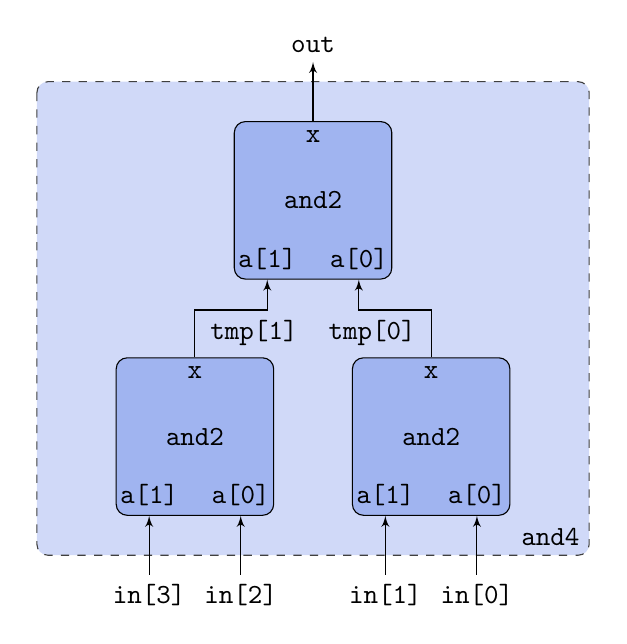
\begin{tikzpicture}[auto, node distance=1.5cm,>=latex',every text node
            part/.style={align=center}]
            \def\blockdist{2em}
            \def\edgedist{2em}

            \begin{pgfonlayer}{foreground}
                \node[block] (top) {\texttt{and2}};
                \node[branch,below of=top,node distance=3cm] (mid) {};
                \node[block,right of=mid] (right) {\texttt{and2}};
                \node[block,left of=mid] (left) {\texttt{and2}};

                \draw[->] (right.north) node[anchor=north] {\texttt{x}} |- +(-0.75cm,0.6cm)
                node[anchor=north] {\texttt{tmp[0]}} -| (top.300) 
                node[anchor=south] {\texttt{a[0]}}; 
                \draw[->] (left.north) node[anchor=north] {\texttt{x}} |- +(+0.75cm,0.6cm) 
                node[anchor=north] {\texttt{tmp[1]}} -| (top.240)
                node[anchor=south] {\texttt{a[1]}}; 
                \draw[<-] (left.240) node[anchor=south] {\texttt{a[1]}} -- +(0cm,-0.75cm)
                node[anchor=north] {\texttt{in[3]}};
                \draw[<-] (left.300) node[anchor=south] {\texttt{a[0]}} -- +(0cm,-0.75cm)
                node[anchor=north] {\texttt{in[2]}};
                \draw[<-] (right.240) node[anchor=south] {\texttt{a[1]}} -- +(0cm,-0.75cm)
                node[anchor=north] {\texttt{in[1]}};
                \draw[<-] (right.300) node[anchor=south] {\texttt{a[0]}} -- +(0cm,-0.75cm)
                node[anchor=north] {\texttt{in[0]}};
                \draw[->] (top.north) node[anchor=north] {\texttt{x}} -- +(0cm,0.75cm) 
                node[anchor=south] {\texttt{out}};
            \end{pgfonlayer}
            \begin{pgfonlayer}{background}
                \path (top.north -| left.west)+(-1,0.5) node (a) {};
                \path (right.east |- right.south)+(1,-0.5) node (b) {};
                \path[fill=RoyalBlue!25, rounded corners, draw=black!75, dashed] (a) rectangle (b);
            \end{pgfonlayer}
            \begin{pgfonlayer}{foreground}
                \draw[] (b) node[anchor=south east] () {\texttt{and4}};
            \end{pgfonlayer}
        \end{tikzpicture}
    \end{figure}
\end{frame}

\section{Lab Assignment}

\begin{frame}{Lab Assignment}
    \begin{itemize}
        \item Follow the tutorial, this is one of the most important documents
            in this class\dots
        \item Assignment on the \href{http://www.eecs.umich.edu/eecs/courses/eecs470}{\underline{course website}}.
        \item Submission: Place yourself on the \href{https://oh.eecs.umich.edu/courses/eecs470}{\underline{help queue}} and we will check you off when you feel comfortable you can demonstrate what is required
    \end{itemize}
\end{frame}

\begin{frame}{Useful Links}
    \begin{itemize}
        \item Recordings can be found on \href{https://piazza.com/class/kjoqguntyr139?cid=7}{\underline{piazza}}
        \item Consider using \href{https://docs.google.com/document/d/1xtkhDykp9vtkyjXg_1e1PFLRxDDjNmuUWUHt-wfaDjU/edit?usp=sharing}{\underline{VS Code with Remote SSH}} via Scott's helpful guide
        \item Get comfortable using \href{https://caenfaq.engin.umich.edu/linux-login/how-do-i-connect-to-a-caen-linux-computer-remotely}{\underline{CAEN VNC}} if you can 
        \item Review the \href{https://docs.google.com/document/d/1U9FOOYAPqvhSQda-v66SCmUgdvuaBs1KIK8Ht4_WSCA/edit?usp=sharing}{\underline{GTKwave Waveform Viewer tutorial}} should VNC be too delayed
        \item Read the  \href{https://docs.google.com/document/d/1mnxgtQkvPcpKlBzCL9bKiwrFYpbx-hsqfRTPK-weB7Q/edit?usp=sharing}{\underline{Screen tutorial}} before synthesizing your projects.
        \item Assignment on the \href{http://www.eecs.umich.edu/eecs/courses/eecs470}{\underline{course website}}.
        \item Submission: Place yourself on the \href{https://oh.eecs.umich.edu/courses/eecs470}{\underline{help queue}} and we will check you off.
    \end{itemize}
\end{frame}

\appendix
\end{document}

